\section{Noise Generation}

When evaluating image processing algorithms, it is important to see how they perform under various levels of noise.


\begin{figure}[ht]
\centering
	\subfigure[Original image]{
	
\includegraphics[width=0.45\linewidth]{question2/toy}
	}
\end{figure}


\subsubsection{Describe each of the histograms in the context of the corresponding noise models. Why do they appear that way?}
In the histogram of the Gaussian noised image, pixel intensities are grouped in Gaussian distributions centred around the two intensity values of the original image. It appears this way because Gaussian noise is additive noise. Each pixel in the image is having a value sampled from a Gaussian distribution added to it, with the value added having a mean of zero and a variance of 0.01.

Speckle noise is a multiplicative type of noise. The histogram appears to be a uniform distribution centred around the original intensities. Speckle noise samples from a uniform distribution centred on 1, with a range relating to the specified variance parameter. There is more variance around the higher original intensity value, which is due to the multiplicative nature of speckle noise. Higher values have a higher absolute absolute variance, but they have the same coefficients of variance.

The salt and pepper noise histogram is very similar to the original image, there is also a number of pixels of 0 and 1 intensity that are obscured by the histogram axes.

\begin{eqnarray}
100 \times \left [ 0.9, 1.1 \right ] = \left [ 90, 110 \right ] \\
{\sigma}^{2} = 33.3 \nonumber \\
{c}_{var} = 0.057 \nonumber
\end{eqnarray}

\begin{eqnarray}
200 \times \left [ 0.9, 1.1 \right ] = \left [ 180, 220 \right ] \\
{\sigma}^{2} = 133.3 \nonumber \\
{c}_{var} = 0.057 \nonumber
\end{eqnarray}

\begin{figure}[htcb]
\centering
	\subfigure[Image with Gaussian Noise; $\sigma^2$=0.01]{
	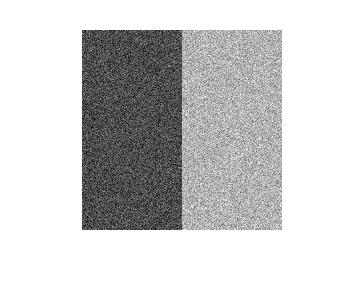
\includegraphics[width=0.45\linewidth]{question2/gauss}
	}
	\subfigure[Histogram of Gaussian Noise Image]{
	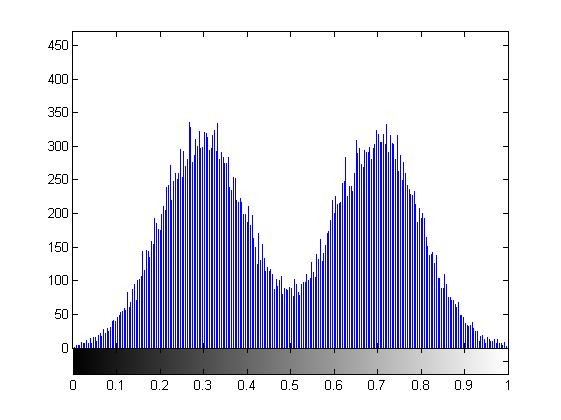
\includegraphics[width=0.45\linewidth]{question2/gauss_hist}
	}
	\subfigure[Image with Speckle Noise; $\sigma^2$=0.04]{
	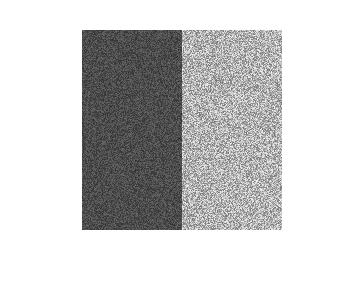
\includegraphics[width=0.45\linewidth]{question2/speckle}
	}
	\subfigure[Histogram of Speckle Noise Image]{
	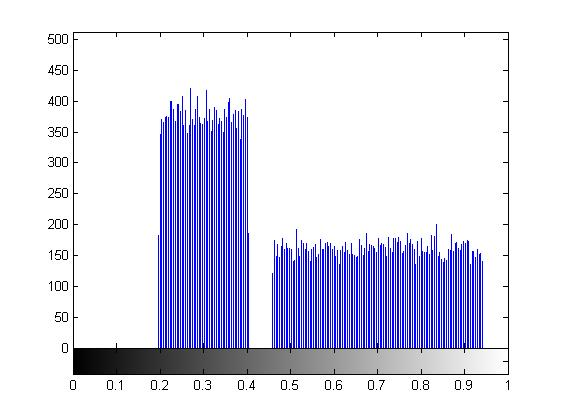
\includegraphics[width=0.45\linewidth]{question2/speckle_hist}
	}
	\subfigure[Image with Salt and Pepper Noise; $\rho$=0.05]{
	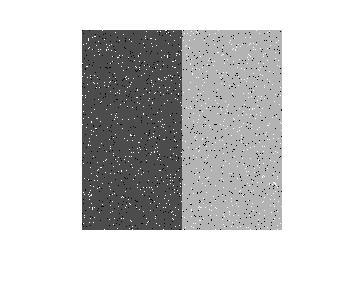
\includegraphics[width=0.45\linewidth]{question2/salt}
	}
	\subfigure[Histogram of Salt and Pepper Image]{
	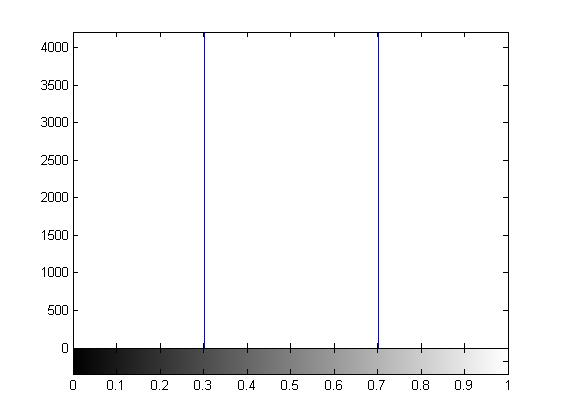
\includegraphics[width=0.45\linewidth]{question2/salt_hist}
	}
	\caption{Toy image with Gaussian, Salt and Pepper, and Speckle Noise}
	\label{fig:noiseGeneration.toy}
\end{figure}
 



\subsubsection{Are there visual differences between the noise contaminated images? What are they? Why?}
There exist some distinct differences between the Gaussian, speckle and salt and pepper noise contaminated images. The Gaussian noised image has a lot more extra bright or extra dark pixels due to the unbounded nature of a Gaussian function can result in a pixel being shifted far from it's original intensity.

The speckled noise image seems to have no pixels at their original intensity, but all pixels have only been slightly perturbed, due to the bounded multiplicative nature of speckle noise.

The salt and pepper noise leaves most of the image unmodified, and changes some of the pixels in the image, in a position invariant method, to with zero or 1.

\subsubsection{In the speckle noise case, what is the underlying distribution used? Can you tell from the histogram? How?}
The underlying distribution of speckle noise is a bounded uniform distribution from which a value is sampled and multiplied by the pixel intensity in question. It is very apparent from the histogram because the intensities around the original image intensities are distributed roughly evenly (i.e. same number of pixels).

\subsubsection{In the speckle noise case, you will notice that the peaks of the histogram are no longer of the same height as they were in the original image. Also, the spread around each of the peaks is also different from each other. Why? Hint: Noise is multiplicative}
Since the noise is multiplicative, it is proportional to the local grey level in the image. i.e. there will be a wider spread of values around higher grey levels, as we can see with the right-most spread having a higher variance.
